\input{preamble}
\usepackage{bytefield}

\hypersetup{
  pdftitle={AAUB\AA D},
  pdfsubject={1st semester Control and Automation, Aalborg University},
  pdfauthor={Rasmus Lundgaard Christensen, Nick Østergaard, Frederik Juul, Atilla, Tudor},
  pdfcreator=LaTeX,
  linkcolor=black,
  citecolor=black,
  filecolor=black,
  urlcolor=black
}

\begin{document}
\chapterstyle{nickoe}
\frontmatter
\author{Nick Østergaard \and Rasmus Lundgaard Christensen \and Frederik Juul \and Attila Fodor \and Todor Muresan}
\title{An autonomous marine environment surveying platform}
\date{\today}
\maketitle
\begin{center}
Worksheet \#3 by group 12gr730
\end{center}



\cleardoublepage
%\input{formalities/titlepage}
%\input{formalities/preface}
%\input{formalities/terminology}

%%%%%%% Maybe we should have an overview of the system here
\cleardoublepage
\tableofcontents


\mainmatter
\documentclass[a4paper,11pt,oneside,fleqn]{article}
% Pakker
\usepackage[utf8]{inputenc} % Så må vi bruge æ, ø og å
%\usepackage[ansinew]{inputenc}
%\usepackage[danish]{babel} % Dansk opsætning
\usepackage[T1]{fontenc} % Hjælper med ordeling ved æ, ø og å. Sætter fontene til at være ps-fonte i stedet for bmp.
\usepackage[english,final]{varioref} % Vi kan anvende \vref
\usepackage{array,booktabs} % Til gode tabeller
\usepackage{acronym} % Smart akronymhåndtering
\usepackage{minitoc} % Vi kan lave del inholdsfortegnelser forhåbentlig
\usepackage{graphicx} % We can now use \includegraphics and stuff
\usepackage{pdfpages} % Inkludere en pdf side som en side  
\usepackage{bytefield}


\begin{document}
\author{Nick Østergaard \and Rasmus Lundgaard Christensen \and Frederik Juul \and Attila Frodor \and Todor Muresan}
\title{An autonomous marine environment surveying platform}
\date{\today}
\maketitle
\begin{center}
Worksheet \#1 by group 12gr730
\end{center}

\section{Introduction}
Measuring environmental parameters in and around the water in Greenland (or any watery nation) is a time consuming task. Today measurements are carried out by manually navigating large vessels up and down along the coastline and into the fjords. 

The purposes of these measurements could be to measure the water depth for bathymetric surveys. This would allow for safer voyages in and around the coastlines, and for general environmental studies. 

These measurements are today carried out by one large vessel, which could be exchanged for several smaller ones to reduce the surveying time and labor cost. This would make for a faster measurement of the coastline as well as giving an opportunity to measure previously un-surveyed waters due to costs. 

Reducing the size of a vessel, poses some other challenges in regards to the weather conditions and other environmental parameters, that has a much larger influence on small scale vessels, than on larger ones. This paper will deal with how such a surveying vessel can be developed, and still measure the water depth whilst under the influence of the above.

A challenge using a single beam transducer to measure water depth is the roll/pitch of the craft. Figure \vref{fig:beamer} illustrates this problem, where an induced pitch of the ship (eg. a wave) makes it impossible for the vessel to make a precise measurement.

\begin{figure}[h]
\centering
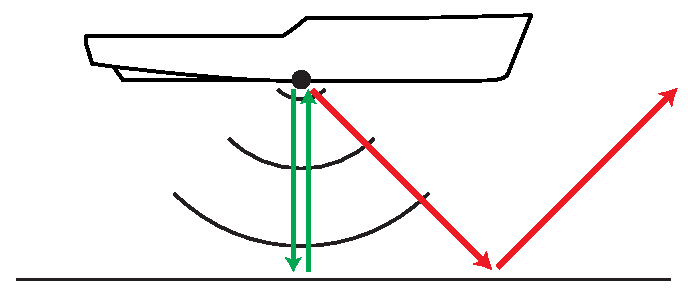
\includegraphics[width=0.5\textwidth]{img/beamer}
\caption{Overview of a depth mapping system. The green represents a measurement shot directly down and the red represents a measurement with induced pitch on the ship}
\label{fig:beamer}
\end{figure}

\end{document}
\section{Platform}
\label{sec:platform}
In this system overview, the platform along with the electronics and its software is described to aid in understanding the physical interconnections that exist between the modules.

The system consists of a wide range of modules which may be sensors or actuators. These modules are connected to a \ac{LLI} and \ac{HLI} computing device. The \ac{LLI} is a microcontroller which takes care of the basic functions of the platform such as communicating with basic sensors and actuators. The software for this is embedded and written in C for the avr-gcc compiler.

The \ac{HLI} is a x86 compatible computer of some sort that is able to run the higher abstraction layer code written in Python. This code implements the onboard generation of waypoints from map data to calculate the desired heading and speed for the vessel. It also implements the state space model and calculates propeller speeds and in turn sends these to the \ac{LLI}.

Some modules that are connected to the \ac{LLI} are not handled by the \ac{LLI} itself, but instead it forwards the data to the \ac{HLI} which uses it for the control algorithm. A illustration of this can be seen on figure~\vref{fig:vessel-block-overview}.

\begin{figure}[htbp]
	\centering
	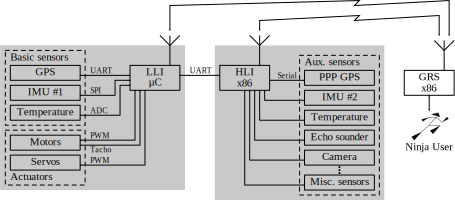
\includegraphics[width=\textwidth]{img/vessel-block-overview-electrical}
	\caption{Overview of electrical interconnections between \ac{LLI} and \ac{HLI} together with periphal modules.}
	\label{fig:vessel-block-overview-electrical}
\end{figure}

\chapter{FAPS LLI interface}
\head{Documentation for the LLI part of the system.}
\section{Standard format of messages}
%To develop a suiting protocol for AAUSHIP1, the data to be sent via this is looked at in more detail in section~\vref{sec:lli-bandwith}. For instance, the \ac{IMU} has serveral different outputs, and receiving them all in one big stream might increase the load on the network, so splitting these up could free up some bandwidth which could be used for other (and more important) tasks. \todo{How can the last statement be true?}

To develop a suiting protocol for AAUSHIP1, the data to be sent via this is looked at in more detail in section ~\vref{sec:lli-bandwith}. For instance, the \ac{IMU} has several different outputs, which needs to be processed independent of each other. Because of this, they are broken into separate packages, each with their own ID and checksum. This simplifies parsing and allows the protocol to easily be expanded to other sensors and actuators which were not included in the original design. A short, single state packet limits the effect of a flipped bit, since only a single state has been lost, compared to a packet containing all information.

As both the \ac{IMU} and \ac{GPS} is sending packets of varying size, the data field in the protocol should be variable. However, there are some fixed elements, which is possible to decide now. The number of sensors/actuators connected to the \ac{LLI} can by design not be more than 256, which makes way for a 1-byte device resolution. As each device might contain several outputs (as seen from the \ac{IMU}) each device ID is then given an additional byte for message IDs. In addition to this header a length byte is contained to describe the length of the data field, to make it easier to parse. Lastly a \ac{CRC} checksum is added on the end to verify the content. Figure~\vref{fig:bytefield} depicts the packet structure. Everything other than the data field is fixed length as described in table~\vref{tab:general}. 
The data field can be either binary or ASCII, depending on the source. It is desired to limit the amount of calculations necessary at the LLI, seeing as the power of the HLI is many times greater, as well as the implementation being simpler.

\begin{figure}[h]
\centering
\begin{bytefield}{30}
\begin{rightwordgroup}{Header}
\raisebox{-1mm}{$\underbrace{\raisebox{1mm} {\bitbox{1}{\texttt{\$}}  \bitbox{5}{Length}   \bitbox{5}{DevID} \bitbox{5}{MsgID}}}_\mathrm{Header}$}%
\raisebox{-1mm}{$\underbrace{\raisebox{1mm} {\bitbox{16}{Data field }}}_\mathrm{Variable\ length}$}\bitbox{4}{CRC16} 
\end{bytefield}
\caption{Generic message bytefield}
\label{fig:bytefield}
\end{figure}

%The packet bytes are arranged as little endian (MSB first), and such should the numbering og bytes also be, i.e. the start start characther comes first when transmitted and ends with the end character which is the newline character.

The packet bytes are little endian (MSB first), which is consistent throughout the packet. The data field is arranged as always being a full number of bytes, to simplify transmission and receiving. This conforms to the RS232 standard.

\begin{table}[htbp],
	\centering
	\begin{tabular}{llll}
		\toprule
		\textbf{Field name} & \textbf{Size [bytes]} & \textbf{Type} & \textbf{Description}\\
		\midrule
		Startchar & 1 & uint8 & Start character (\texttt{\$}) \\
		Length & 1 & uint8 & Length of data field in the range 1--250\\
		DevID & 1 & uint8 & Device identifier \\
		MsgID & 1 & uint8 & Message identifier \\
		Data & 1--250 & uint8 & Data portion (binary or ASCII )\\
		Checksum & 2 & uint8 & CRC-16 checksum on data part \\

		\bottomrule
	\end{tabular}
	\caption{General description of the packet format}
	\label{tab:general}
\end{table}

The device ID (DevID) also serves as the priority of the packets, enabling more important packages to be sent prior to less important ones. For example; auxillaury parameters as temperature measurements are less important in time than navigational informations from the \ac{IMU} which has to be precisely known in time and preferably periodically.

\section{Message definitions}
%This is the list of all supported messages for the LLI interface. The messages is the interface to every thing that could be of interest for the HLI, i.e. sensor measurements and actuator control. The list of field descriptions in the following ommits the generic fields, with start character and checksum.
The initial list of supported devices and message IDs is given in table TODO. The initial devices are distributed evenly with 10 IDs between each device to allow for other new devices to be implemented with with lower, higher priority, IDs. The general functions of the LLI are implemented with the highest available priority, since it has the deadman switch implemented but a very low amount of regular activity.
From the definition of the DevID and MsgID each packet can be identified as having to do with a given part of the system. This is the same throughout the system. For some parts of the system, such as the motors, it is not possible to see whether the packet is a set or a get command, from the initial data structure. To mediate this, a "Read thruster" command is implemented, and should be implemented for all future actuators or other devices which are not just passively feeding back data. This would be achieved by sending a "Read thruster" packet to the LLI from the HLI. The LLI will neglect the data part of this message, as it unnecessary to understand the intention of the package. It will then respond with the MsgID and  DevID, but with the data is has read from the MotorSpeed register.
To facilitate the Plug and Play nature of the system, the first 3 available MsgIDs are defined to have a set meaning. These are given in table TODO.
\begin{table}[h]
\centering
\begin{tabular}{ll}
\toprule
\textbf{MsgID} & \textbf{Definition}\\
\midrule
0 & List available MsgIDs along with their functionality\\
1 & Set options for device\\
2 & Read options from device\\
\bottomrule
\end{tabular}
\end{table}
 If a packet with MsgID 0 is sent to a device, the device will respond with a list of all available MsgIDs, along with their definition. If a packet with MsgID 0 is sent to DevID 0, the General LLI, it will respond with a list of available devices. If these device definitions adhere to a strict protocol, it will be possible to automatically configure an LLI and HLI implementing this protocol. This protocol will not be defined in this project, but the feature will useful in checking and validating the configuration.
\begin{table}[h]
\centering
	\begin{tabular}{lllll}
	\toprule
	& \textbf{Message Name} & \textbf{MsgID} & \textbf{Data Size} & \textbf{Contains}\\
	\midrule
	\multicolumn{5}{l}{\textbf{0: General}}\\
	\midrule
	& Deadman Switch & 0 & 1 & On or off signal for actuators \\
	& Status & 1 & 250 & Statuses of sensors and actuators \\
	& Ping & 2 & 0 & Empty \\
	& Pong & 3 & 0 & Empty \\
	& ACK & 4 & 0 & Empty \\
	& NACK & 5 & 0 & Empty \\
	& Build Info & 6 & 250 & Commit, target, date\\
	& Surge & 7 & 1 & Speed\\
	& Turn & 8 & 1 & Turning velocity\\
	\midrule
	\multicolumn{5}{l}{\textbf{10: Actuators}}\\
	\midrule
	& Set thruster & 0 & 2 & Desired Speed\\
	& Read thruster & 1 & 2 & Set Speed \\
	& Set left thruster & 2 & 2 & Desired Speed\\
	& Read thruster & 3 & 2 & Set Speed\\
	& Set bow thruster & 4 & 2 & Desired Speed\\
	& Read bow thruster & 5 & 2 & Set Speed\\ 
	\midrule
	\multicolumn{5}{l}{\textbf{20: IMU}}\\
	\midrule
	& X-Acceleration & 0 & 2 & Acceleration in X-direction\\
	& Y-Acceleration & 1 & 2 & Acceleration in Y-direction\\
	& Z-Acceleration & 2 & 2 & Acceleration in Z-direction\\
	& X-Gyro & 3 & 2 & Gyroscope in X-direction\\
	& Y-Gyro & 4 & 2 & Gyroscope in Y-direction\\
	& Z-Gyro & 5 & 2 & Gyroscope in Z-direction\\
	& X-Mag & 6 & 2 & Magnetometer in X-direction\\
	& Y-Mag & 7 & 2 & Magnetometer in Y-direction\\
	& Z-Mag & 8 & 2 & Magnetometer in Z-direction\\
	& Temp & 9 & 2 & Temperature in IMU\\
	\midrule
	\multicolumn{5}{l}{\textbf{30: GPS}}\\
	\midrule
	& Velocity & 0 & 2 & Velocity\\
	& Latitude & 1 & 4 & Latitude\\
	& Longitude & 2 & 4 & Longitude\\
	\midrule
	\multicolumn{5}{l}{\textbf{40: Temperature}}\\
	\midrule
	& Temp 0 & 0 & 2 & Temperature \\
	& Temp 1 & 1 & 2 & Temperature \\
	& Temp 2 & 2 & 2 & Temperature \\
	\midrule
	\multicolumn{5}{l}{\textbf{50: Voltage}}\\
	\midrule
	\bottomrule
	\end{tabular}
\end{table}

\section{General messages}

\begin{table}[h]
	\centering
	\begin{tabular}{llll}
		\toprule
		\textbf{Message name}  & \textbf{msgid} & \textbf{data size} & \textbf{Action}\\
		\midrule
		Deadman switch & 0 & 1 & Turn on or off actuators and wait for manual control \\
		Status of system & 1 & 250 & Statuses of sensors and actuators \\
		Ping & 2 & Empty \\
		Pong & 3& Empty \\
		ACK & 4 & Empty\\
		NACK & 5 & Empty\\
		Build info & 6 & 250 & Commit, target, date\\
		Surge & 7 & 1 &\\
		Turn & 8 & 1 &\\
		\bottomrule
	\end{tabular}
	\caption{Byte field description of general messages (devid 0)}
	\label{tab:ack}
\end{table}

\todo{Expand each message row with rows of data fields}

\section{Actuator messages}
\begin{table}[h]
	\centering
	\begin{tabular}{llll}
		\toprule
		\textbf{Message name}  & \textbf{msgid} & \textbf{data size} & \textbf{Action}\\
		\midrule
		Actuators ON/OFF & 0 & 1 & Bit mask representing which actuators should be of and on\\
		Set right thruster & 1 & 2 & Speed (main trhuster of only one) \\
		Set left thruster & 2 & 2 & Speed \\
		Set bow thruster & 3 & 2 & Speed \\
		\bottomrule
	\end{tabular}
	\caption{Byte field description of actuator messages (devid 1)}
	\label{tab:ack}
\end{table}

\section{Sensor messages}
\begin{table}[h]
	\centering
	\begin{tabular}{llll}
		\toprule
		\textbf{Message name}  & \textbf{msgid} & \textbf{data size} & \textbf{Action}\\
		\midrule
		Acclerometer & 0 & 1 & \\
		Gyrometer & 1 & 2 & \\
		Magnetometer & 2 & 2 &  \\
		GPS & 3 & 2 & GPGGA data \\
		\bottomrule
	\end{tabular}
	\caption{Byte field description of sensor messages (devid 3)}
	\label{tab:ack}
\end{table}




STATUS
gps
vsupply
under\_way
actuators\_on
autopilot\_on
cpu\_usage

ACTUATORS\_OFF

ACTUATORS\_ON

MARK\_HOME

GET\_POSITION

REPORT\_POSITION


\section{Analysis of data and bandwidth}
\label{sec:lli-bandwith}
To be able to evaluate if there is enough bandwidth on between the serial connections from LLI, HLI and ground station, an analysis is hereby conducted.


\section{Frames of reference}
There are different frames of reference, which is defined here. There are the global frame which is the the earth, this frame operates in various coordinate systems such as the \ac{WGS84} and \ac{ECEF}. In addition to this there is a local frame/inerital frame, which is a tangential plane on the surface of the earth int he area the vessel has to operate. Lastly the vessel has a frame attached to this, which is the body frame. All x,y,z frames are righthanded.

\begin{figure}[htbp]
	\centering
	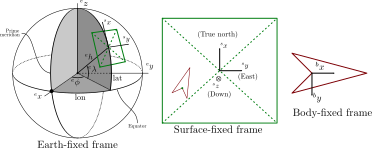
\includegraphics[width=\textwidth]{img/reference_frames}
	\caption{Definitions of the reference frames, using the same system as \cite{argo}.}
	\label{fig:vessel-block-overview}
\end{figure}

\todo{Rotation matrices could be of interest here, but see \cite{argo} for now.}

\section{Autonomous control}
\begin{frame}{System levels}
    \includegraphics[width = \textwidth]{control/img/vessel-block-overview}
\end{frame}

\begin{frame}{HLI features}
		\begin{itemize}
			\item Model-based development that allows multiple Ship instances
			\centering
			\includegraphics[trim = 5mm 5mm 5mm 5mm, clip, width = 0.8\textwidth]{control/img/actor-model}
			\item Seamlessly integrated custom Simulation environment
			\centering
			\includegraphics[trim = 5mm 5mm 5mm 5mm, clip, width = 0.8\textwidth]{control/img/simmodel}
		\end{itemize}
\end{frame}
%%%%%%%%%%%%%%%%

\subsection{Path Planning}
\begin{frame}{Waypoints and Sub-Waypoints}
    \begin{block}{Waypoints}
		\begin{itemize}
			\item Key points of interest, defining the \textbf{approximate path}
			\item Coastal information \textbf{known} $\rightarrow$ \textbf{automatic} WP generation
			\item Coastal information \textbf{unknown} $\rightarrow$ \textbf{manual} WP placement
		\end{itemize}
    \end{block}
    \begin{block}{Sub-Waypoints}
		\begin{itemize}
			\item Specific locations that the ship must approach
			\item Placed in the $\lambda_{max}$ surrounding of the \textbf{approximate path}
			\item The ship approaches each \textbf{SWP} at least to $\varepsilon$ \textbf{follow distance}
			\item Each Waypoint is approached to \textbf{at least} $\lambda + \varepsilon$ distance
		\end{itemize}
	\end{block}
\end{frame}
%%%%%%%%%%%%%%%%

\begin{frame}{Local path planning}
		\begin{itemize}
			\item Key points are determined to define an \textbf{Euler Spiral} $\rightarrow$ \textbf{Circular} $\rightarrow$ \textbf{Euler Spiral} path
			\item The centrifugal force affecting the body of the ship changes continuously and linearly
			\item The resulting sideways-movement is kept to a minimum and the control signal is better conditioned
		\end{itemize}
			\begin{tabular}{l l}
			\hspace{-3.1mm}
				\begin{minipage}{0.6\textwidth}
					\begin{itemize}
						\vspace{-2.5mm}
						\item The path is populated with Sub-Waypoints and transformed to the proper position on the map 
						\includegraphics[width = \textwidth]{control/img/positioning1}
					\end{itemize}
				\end{minipage}
			&
				\begin{minipage}{0.3\textwidth}
					\includegraphics[width = \textwidth]{control/img/positioning2}
				\end{minipage}
			\end{tabular}
			
		
\end{frame}
%%%%%%%%%%%%%%%%

%%%%%%%%%%%%%%%%
\subsection{Ship Model}
\begin{frame}{Modeling}{System Dynamics}
The Dynamics of the system are given by the drag the ship experiences when moving through the water. The drag is given as:
\begin{align}
F_\text{Drag}(\dot{x},\dot{y}) = \frac{1}{2} \cdot \rho \cdot C_\text{D} \cdot \dot{x}^2 \cdot A 
\end{align}
The formula changes when the ship is turning, as the drag then is converted into a torque - which is defined as:
\begin{align}
\tau_\text{Drag}(\omega) = \frac{1}{2} \cdot \rho \cdot C_\text{D} \cdot (d \cdot (r_f^4 + r_b^4)) \cdot \omega^2
\end{align}
The above can be put an matrix form as:
\begin{align}
\mathbf{A}\mathbf{x} = \begin{bmatrix}
-\beta_X & 0 & 0\\
0 & -\beta_Y & 0\\
0 & 0 & -\beta_\omega
\end{bmatrix}\begin{bmatrix}
\dot{x}\\
\dot{y}\\
\dot{\theta}
\end{bmatrix}
\end{align}
\end{frame}

%%%%%%%%%%%%%%%%
\begin{frame}{Modeling}{System Dynamics}
As the motion in the $y$-direction is uncontrollable, and the thing to be controlled is the velocity and the angle, the combined system becomes:
\begin{align}
\dot{\mathbf{x}} &= \mathbf{A}\mathbf{x} + \mathbf{B}\mathbf{u}\\
\begin{bmatrix}
\ddot{x}\\
\dot{\theta}\\
\dot{\omega}
\end{bmatrix} &= \begin{bmatrix}
\frac{-\beta_x}{m} & 0 & 0\\
0 & 0 & 1\\
0 & 0 & \frac{-\beta_\omega}{I}
\end{bmatrix}\begin{bmatrix}
\dot{x}\\
\theta\\
\omega
\end{bmatrix} + \begin{bmatrix}
\frac{1}{m} & 0\\
0 & 0\\
0 & \frac{1}{I}
\end{bmatrix}\begin{bmatrix}
F_\text{total}\\
\tau
\end{bmatrix}
\end{align}
And the output of the system $\mathbf{y}$ becomes:
\begin{align}
\mathbf{y} &= \mathbf{C}\mathbf{x} + D\mathbf{u}\\
\begin{bmatrix}
\dot{x}\\
\theta\\
\end{bmatrix} &= \begin{bmatrix}
 1 & 0 & 0\\
 0 & 1 & 0
\end{bmatrix}\begin{bmatrix}
\dot{x}\\
\theta\\
\omega
\end{bmatrix} + \mathbf{0}\begin{bmatrix}
F_\text{total}\\
\tau
\end{bmatrix}
\end{align}
\end{frame}

\subsection{Control system}
\begin{frame}{Navigation}
    \begin{block}{Navigation}
		\begin{tabular}{l l}
		\begin{minipage}{0.45\textwidth}
		\begin{itemize}
			\item The ship is always heading for the next Sub-Waypoint, outside of the $\varepsilon$ \textbf{follow distance}
			\item The output of the Navigator is the \textbf{reference heading} $\Theta_r$
			\item The image shows a simulation of the navigation and control based on noisy inputs
		\end{itemize}
		\end{minipage}
		&
		\begin{minipage}{0.50\textwidth}
		\includegraphics[width=\textwidth,keepaspectratio]{control/img/navi}
		\end{minipage}
		\end{tabular}
    \end{block}
\end{frame}

\begin{frame}{Engine controller}
    \begin{block}{Navigation}
		\begin{itemize}
			\item The engine controller is based on the linearized State-Space model
			\item Overview of the control system:
		\end{itemize}
		\includegraphics[trim = 0mm 21cm 0mm 0mm, clip, width=\textwidth]{control/img/controlloop}
    \end{block}
\end{frame}
%%%%%%%%%%%%%%%%
\chapter{Modelling of Twin Screw Ship}
When modelling the forces affecting a \ac{TSS} there few parameters which affect the movement of the ship. These are the forces applied by the motors, as well as the placement of the motors. For calculating these contributions simple trigonometric functions can be used. This gives the resulting forces in the boats X and Y directions, as well as the torque generated.
\begin{figure}
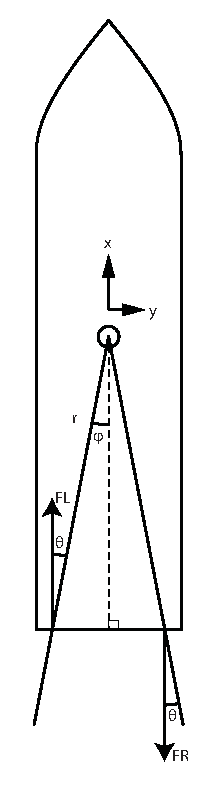
\includegraphics{img/boatmodel.pdf}[h]
\caption{By controlling FL and FR, it is possible to control the translational and rotational forces of the ship. The division of these forces is dependant on the angle of attack, $\theta$.}
\end{figure}
First we see that the boat is mirrored along it's X axis. From this we can set $\theta = \theta_L = \theta_R$ and $\phi = \phi_L = \phi_R$.  Now we have the forces, $F_L$ and $F_R$, as the controllable input to our system. These will be divided as into $F_X$, $F_Y$ and $\tau$, which are the variables that we wish to control. This division takes the form as seen in equation \eqref{Forceequation}.

\begin{equation}
\left[
\begin{matrix}
F_x\\
F_y\\
\tau
\end{matrix}
\right]
 =
 \left[
\begin{matrix}
\cos(\phi - \theta)\\
\sin(\phi - \theta)\\
\sin(\theta) \cdot r
\end{matrix}
\right]
\cdot F_R
+
 \left[
\begin{matrix}
\cos(\phi - \theta)\\
\sin(\phi - \theta)\\
-\sin(\theta) \cdot r
\end{matrix}
\right]
\cdot
F_L
\label{Forceequation}
\end{equation}
We observe that the motors will deliver force parallel to the x-axis, we can further set $\theta = \phi$. If this is the case $\sin(\theta - \phi)=0$, which nullifies the $F_Y$ term, and $\cos(\theta-\phi) = 1 \Longrightarrow F_X = F_L+F_R$ . The forces can then be modelled as equation \eqref{shortformforces}.
\begin{equation}
\left[\begin{matrix}
F_X\\
\tau
\end{matrix}
\right]
= 
\left[
\begin{matrix}
1\\
\sin(\theta)\cdot r
\end{matrix}
\right]
\cdot F_R
+ 
\left[
\begin{matrix}
1\\
-\sin(\theta)\cdot r
\end{matrix}
\right]
\cdot F_L
\label{shortformforces}
\end{equation}

\section{State Space form}
For better control of the system, it is desired to have the model of the ship in State Space form. This makes it possible to design an observer and a controller, which further makes it possible to design poles and zeros of the system.

The state space form for the system has the general form 
\begin{figure}[h]

\begin{equation}
\dot{x}=Ax+Bu
\end{equation}
\begin{equation}
y=Cx+Du
\end{equation}
\begin{tabbing}
Where \= $x$ is the state vector.\\
	\> $\dot{x}$ is the derivative of the state vector.\\
	\> $A$ is the state matrix\\
	\> $B$ is the input matrix\\
	\> $y$ is the output vector\\
	\> $C$ is the output matrix\\
	\> $D$ is the feedforward matrix
	
	
\end{tabbing}
\end{figure}

\section{Position estimation}
To give a better position estimate which can be fed to the controller as well, the different data collected from the sensors mounted are put through a Kalman filter. This filter takes the different measurements as inputs, and uses these to give a better estimate of the position, rather than the quite noisy measurements taken using just the raw \ac{GPS} data. 

To develop such a filter, the model of the ship is to be computed, as well as a mapping of the different inputs and outputs to the system. The model of the forward and sidewards case (surge and sway) are the same as for the discrete system. 

\subsection{State model}
The state model is used as a base for computing the influence the different inputs have on the system. The matrix is the same as the $\vec{A}$ matrix used to describe the state space representation of the system. The general state expression is given as:
\begin{align}
\vec{Y}(n) = \vec{A}(n)\vec{Y}(n-1) + \vec{Z}(n)
\end{align}
\noindent Where:
\begin{ffk}
$\vec{A}(n)$ is the state matrix\\
$\vec{Y}(n-1)$ is the last input to the system\\
$\vec{Z}(n)$ is the driving noise
\end{ffk}
In this case, the driving noise $\vec{Z}(n)$ will be the inputs to the system, which can then be used to estimate the different states. The states to be estimated is the velocity $\dot{x}$, the angular velocity $\omega$ and the angle of the vessel in the local frame $\theta$. The driving noise (or input) can be defined as the $\vec{B}$ matrix in the state system, multiplied with the different inputs given to the system, namely $n_1$ and $n_2$. When inserted, the formula for the state model becomes:
\begin{align}
\vec{Y}(n) = \vec{A}(n)\vec{Y}(n-1) + \vec{B}\vec{u}
\end{align}
And when terms are inserted, the formula becomes: 
\begin{align}
\vec{Y}(n) = \vec{A}(n)\vec{Y}(n-1) + \vec{B}\vec{u}
\end{align}\todo{insert true formula -lunde}

\subsection{Observation model}
The observation model, is a model that models the different observations. In this case, the different observations are measured directly, as we can measure both the angular velocity, the angle and the velocity of the craft. The general formula for the observation model is given as:
\begin{align}
\vec{X}(n) = \vec{H}(n)\vec{Y}(n) + \vec{W}(n)
\end{align}
\noindent Where:
\begin{ffk}
$\vec{H}(n)$ is the model linking the measurements to the observations\\
$\vec{W}(n)$ is the noise from the measurements
\end{ffk}
The noise from the measurements is estimated using previous measurements which can be used to estimate the variance and the mean of the measurements. The noise can in general be seen as zero-mean Gaussian white noise processes, which makes for the assumption:
\begin{align}
\vec{W}(n) \sim \mathcal{N}(0,\sigma_Z^2)
\end{align}
As $\vec{Y}(n)$ is a row vector, $\vec{W}(n)$ is also a row vector with the same dimension. This calls for different variances on the different noise additions, for each of the measurements. As the variance of the noise on the \ac{IMU} is a lot bigger than on the \ac{GPS}. As all the measurements are available directly, the $\vec{H}(n)$ matrix is equal to identity. Giving the final observation model:
\begin{align}
\vec{X}(n) = \vec{Y}(n) + \vec{W}(n)
\end{align}

% Wouldn't it be a fair assumption that a GPS doesn't have zero-mean, but has a wandering mean that would wander over time? 

% Text about the vector Kalman filer
% Text about the covariance matrix of such a system
\subsection{The Covariance matrix}
As the Kalman filter is given as a vector Kalman filter, the covariance matrix is to be computed. The definition for a covariance matrix is given as:
\begin{align}
\mathcal{C} = \text{E}\langle[x(t_1) - \text{E}[x(t_1)]][x(t_2) - \text{E}[x(t_2)]]^\text{T}\rangle
\end{align}
% Text about some simulations of the system
% Text about linearizations / further computation.

\subsection{Position estimation}
This section will contain the different things we've considered during the miniproject in Kalman filtering, and will be used to give a better estimate of the actual position!
Inputs from the \ac{GPS} (position x,y) and velocity
Inputs from the \ac{IMU}
Basically a description of the miniproject. 
\chapter{Hardware considerations}

Because of the practical nature of the project, a wide range of components had to be chosen. There are several things to be taken into consideration when designing a scale ship from scratch

\section{LLI electronics}
The \ac{LLI} electronics is a plug and play device that controls several smaller ship instances. It provides outputs to control the actuators and motors as well as basic sensor readings to the \ac{HLI}.

The \ac{LLI} has been designed to allow for the above functionality. As described in section~\vref{sec:platform} the \ac{LLI} is an embedded platform, for which an Atmel AVR microcontroller has been chosen. The main control board is an Arduino Mega 2560, and a shield interface to all peripherals has been designed~\vref{chap:schema}.

The final LLI supports the following features:
\begin{description}
\item[Serial]\hfill \\ interface to the \ac{HLI} with a baud rate of 115200 bps
\item[PWM]\hfill \\ outputs for actuators
\item[I$^2$C]\hfill \\ option for aux communication
\item[Analog]\hfill \\ inputs for various sensors
\item[Relay driver]\hfill \\ output
\item[5V]\hfill \\ regulated output
\end{description}

More detailed information about hardware layout~\vref{fig:lli-hw} and the hardware schematic~\vref{chap:schema} can be found in the appendix.

\section{Lithium Polymer batteries}

	Lithium Polymer batteries have been chosen for powering the boat motors as well as for all the electronics, because they offer a very high specific energy and energy density, and can be charged in a relatively short period of time. 

\subsection{Energy calculations}
	
	Each battery is composed of 4 series connected cells with a nominal voltage of 3.7 V, making a total of 14.8 V per battery. There will be 6 such units, each storing 3200 mAh worth of charge, which yields a total of $ 6 \cdot 14.8 \text{ V} \cdot 3.2\text{ Ah} = 284.16 \text{ Wh} $, around 1 MJ of energy.
	
	There are two separate electrical circuits: a power circuit for the motors for which there are 4 dedicated batteries connected in parallel and 2 in the electronics circuit which is separated in order to avoid noise in the digital circuitry. These systems are alloted 198.44 Wh and 94.72 Wh respectively.
	
	If the batteries run at full power (draining a maximum of 80 Amps) the ship will be able to sail for 5 minutes, however, a scenario where the engine runs at full power with a brake on the propellers is extremely unlikely.
	
	Measurements show that the engines should be ran at a setting of 60 of the maximum range of 500 (discretized control steps) and that in this case they drain 2.5 A combined. This will give an operation time of 5.1 hours - thus giving quite a big range on the ships. Assuming a 1 m/s velocity kept constant for 2.5 hours, this gives a range of 9 kilometers forth and 9 kilometers back or being able to measure an area of 1 x 1 km in strips 100 meters apart and still have surplus power.
	
	\subsection{Battery care and charge meters}
	
	Due to the delicate nature of Li-Po batteries, it is absolutely required to never over-charge or over-discharge them because there is a high risk of permanent damage to the batteries. If the temperature continues to raise, there is even a risk of fire and/or explosion. In order to prevent this, we are using a dedicated Li-Po charger with an included balancer, which ensures that none of the cells in the batteries go above the absolute maximum of 4.2 V while charging.
	
	The problem of over-discharge is solved in the power circuit due to the fact that the brushless motor controller has a safety switch which does not allow any cell to drop below 3 V, which would cause permanent damage to the batteries, as they cannot recover after being over-discharged. 
	
	The electronic circuit can drain the batteries more than the maximum limit though. In order to prevent this from happening, we implemented a couple of battery level monitors that are integrated in the \ac{LLI} module and, which can compute the battery levels, thus allow the user to retrieve the boat in order to charge it. They should also include a master kill switch that can save the batteries as well.

\section{Electronics design}

	\subsection{Bow thruster controller}
	\label{subsec:bow thruster controller}
	
	The bow thruster controller is a circuit whose function is to provide power to the bow thruster, under the control of the \ac{LLI}. This uses a L298 H-bridge connected to a logic gate, so that it can be driven with just two signals: direction and \ac{PWM}.
	
	Another use of this circuit is to provide a lossless voltage level conversion from the batteries' nominal 14.8V to the motor's 7.2V rated voltage. That means that the maximum theoretical duty cycle of the PWM bow thruster control signal is $ 14.8 / 7.2 = 48 \% $. This, however, is not the actual value that will be used, due to the fall time of the L298 chip, which is pretty big at the 1kHz PWM frequency. By using an oscilloscope to measure the True RMS value of the electronic circuit's output, it was empirically determined that the maximum pulse width value is 33\%. 
	The motor used to drive the bow thruster also has a minimum starting voltage for which the PWM minimum duty cycle was empirically determined to be around 5\% in this case.
	
	Since the L298 chip has two H bridges inside it, the designed board which can be viewed in the appendix \vref{appendices:bow thruster schematic} includes the circuitry and parts for the two controllers, since it would provide redundancy in case one of them is overloaded or otherwise stops functioning.
	
\section{Motors and propellers}

As the ship should be able to cope with rather powerful streams a powerful propulsion system had to be chosen. The main propulsion unit consists of 2 Grapuner Brushless 750 14.8 V 1200W engines - which together produce around 3 HP at maximum input. With these powerful engines we have a large dynamic range, that allows for fast acceleration and a fast maneuvering, as well as navigating in strong currents. 

The propellers are 2 counterrotating Raboesch brass propellers with a diameter of 60 mm. 
\chapter{Random notes about LLI concepts}
\includepdf[pages=-]{scans/hlinotes1}
\includepdf[pages=-]{scans/hlinotes2}
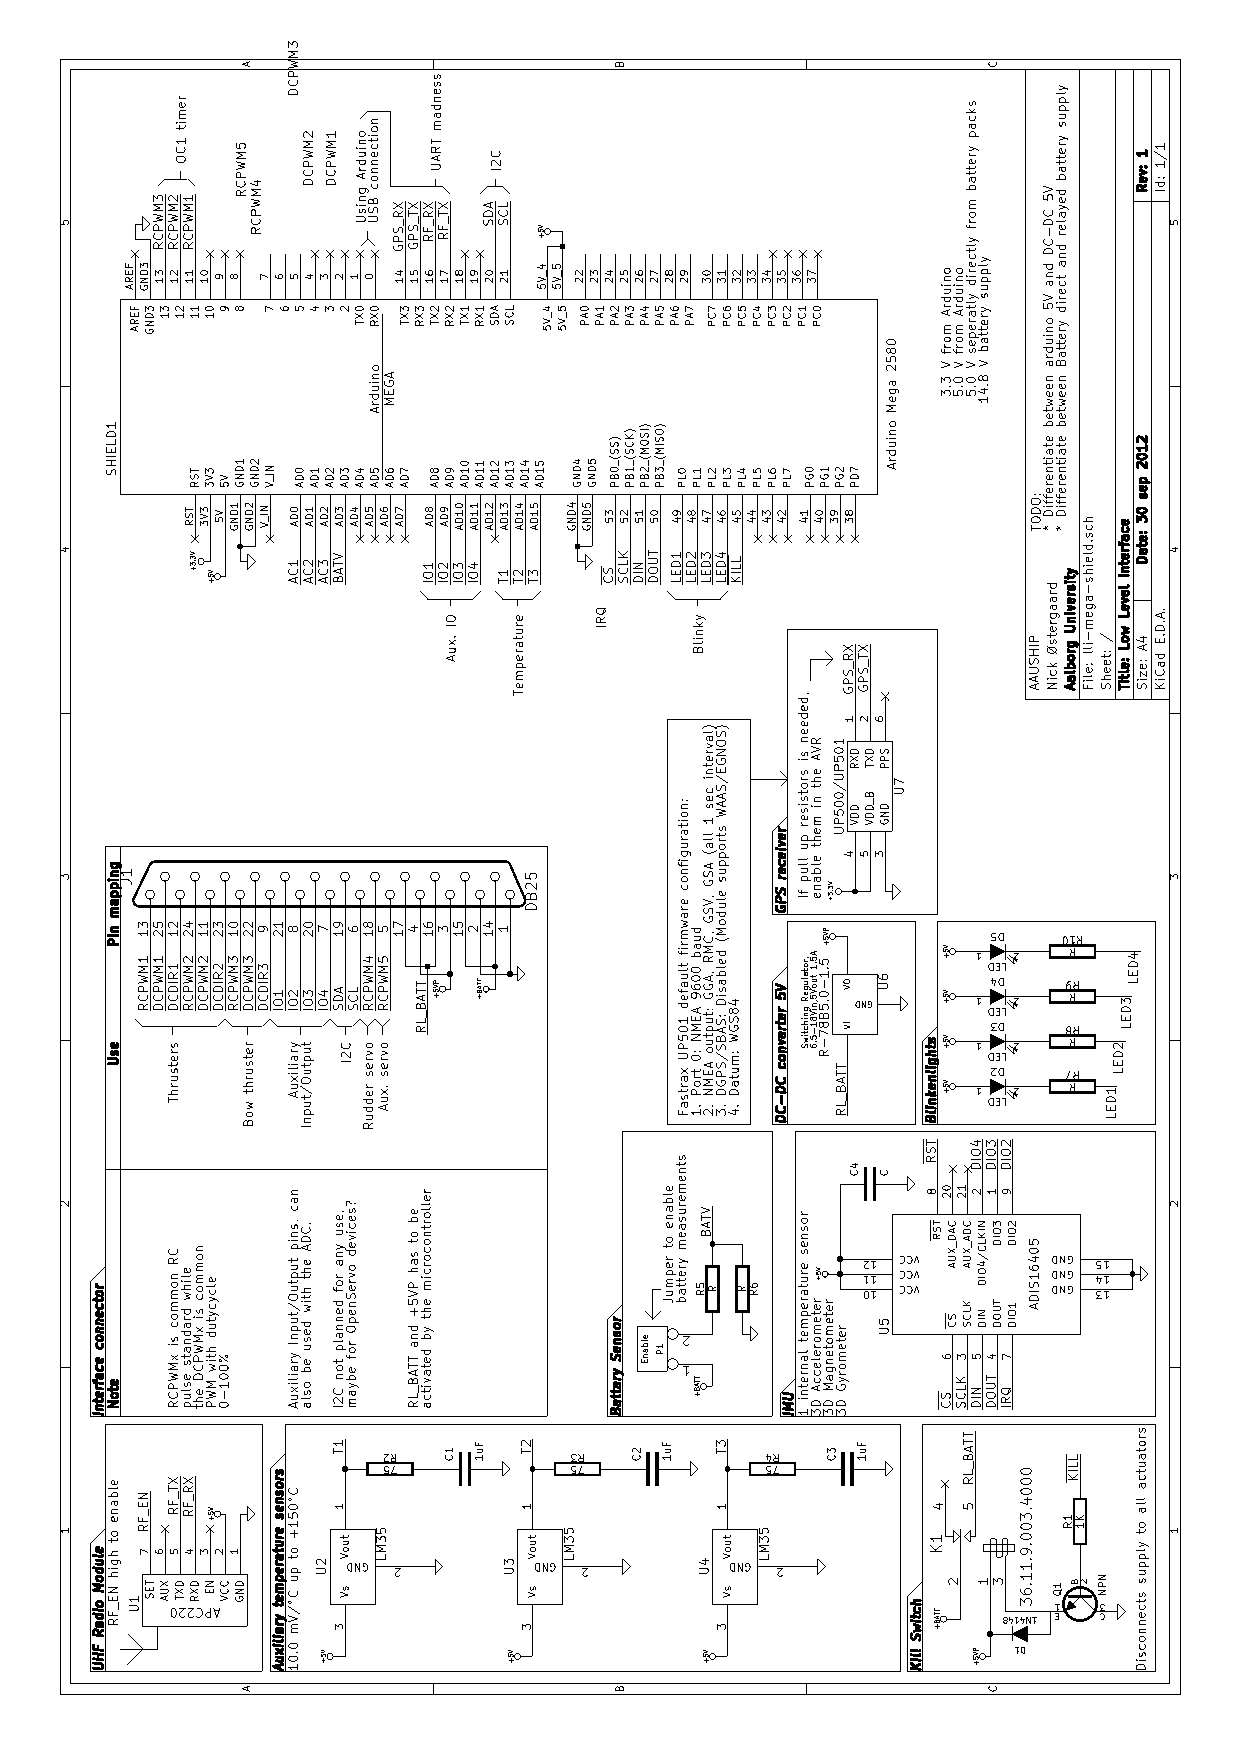
\includepdf{img/lli-mega-shield}


\backmatter
\chapter{Appendix}
\bibliography{litterature}
\label{ch:litt}
\section{List of acronyms}
\begin{acronym}[TDMA]
  \acro{CRC}{Cyclic Redudancy Check}
  \acro{GPS}{Global Positioning System}
  \acro{GRS}{Ground Segment}
  \acro{HLI}{High Level Interface}
  \acro{IMU}{Inertial Measurement Unit}
  \acro{LLI}{Low Level Interface}
  \acro{OSM}{OpenStreetMap}
  \acro{PWM}{Pulse Width Modulation}
  \acro{SSS}{Single Screw Ship}
  \acro{SSM}{State Space Model}
  \acro{TSS}{Twin Screw Ship}
\end{acronym}



%\settocdepth{section}
%\listoftodos
\end{document}

